\chapter{Introduction}
A short general text about the area of ai that your project belongs to.
\\\\
from course page:\\
* Machine learning of statistical classifiers, in this case applied to the task of categorizing documents\\
* Statistical analysis of experiments, such as comparing measurements of classification accuracy.

\section{Background}
* varför är det gött med machine learning? \\
* varför vill vi kunna kategorisera texter?

\section{The problem}
Here you describe the problem in your own words!
\\\\
implementera:\\
* naive bayes\\
* perceptron\\
* average perceptron\\
* knn\\
* (svm)
\\\\
testa:\\
* in-domain sentimental\\
* out-domain sentimental\\
* test categorization
\\\\
features:\\
* unigram\\
* bigram\\
* snowball\\
* tf-idf\\
* stopwords

\section{Theory}
Describe briefly the scientific papers or book chapters you found relevant to the problem, references to sec 6. Explain which are relevant for your project and which not and why.
\\\\
hitta kapitel om\\
* naive bayes\\
* perceptron\\
* knn\\
* svm \\
* text categorization

\subsection{K-nearest neighbors (KNN)}
%http://www.cse.chalmers.se/edu/course/TDA231/mlsli11.pdf
K-nearest neighbors (KNN) algorithm is one of the simplest machine learning
algorithms. The classification performed by KNN works as follows: Fix some
number $k$. For any new $x \in X$, take the most common classification value among
the $k$ training examples in $D$ closest to $x$\cite{ml_2011}.

Even though the KNN algorithm
seems extraordinary simple there are some things that one must take in
consideration. First of all what is nearest? There is of course a natural
distance function in a geometrical space but a proper definition in parameter
space is not obvious. As it turn out a distance function can be defined in a lot
of ways. The given attributes are overall very different in reality.
One may may multiply each attribute variable by arbitrary factors or in other
words stretch the coordinate axes arbitrary and independent. It is very easy to
find examples when doing so will result in very different outcomes of the classifications.
Even further irrelevant attributes may change the classification even though they
shouldn't do so. This phenomena is called \emph{curse of dimensionality}. One
can try to find good stretch factors by performing cross validation.
One takes a vector of stretch factors that
minimizes the classification errors on a valid set. The back side is that
this will require a lot of test vectors\cite{ml_2011}.

An other problem is the computation complexity. KNN is sad to have a lazy
learning method. In other words it does output hypotheses in explicit form.
Instead a lot of computational steps are required for the classification\cite{ml_2011}.

A further issue is to find a suitable $k$. A great choose of $k$ various
depending on many circumstances. A keystone is that if the training set is large
it's important get rid of noise in the data hence increase $k$. On the other
hand a big $k$ requires more calculation. There are however also other more
complex ways for reducing noise \cite{ml_2011}.
%https://dl.dropbox.com/u/5139428/ml-course/Classification1.pdf
\begin{center}
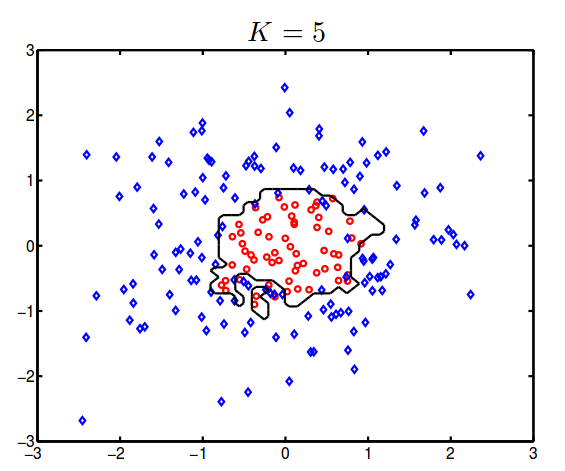
\includegraphics[scale=0.5]{fig/KNN.png}
\end{center}



\subsection{Programs and tools}
What tools and programs are already available for the problem, or for closely related ones?
Describe these briefly. Say how you can use them, and how your work will build on them, or differ from them. Explain which are relevant for your project and which not and why.
\\\\
* vilka program är vettiga att använda? -leta upp några-fördelar/nackdelar
skriv att vi valde matlab och varför.

